\section{Proponowany zakres}

\subsection{Implementacja symulacji chmary}
Projekt zakłada stworzenie programu obrazującego zachowanie chmary.
Chmara będzie zaimplementowana wykorzystując model Craiga Reynoldsa
\cite{reynolds}. Wszystkie obliczenia niezbędne do przeprowadzenia i rysowania
symulacji będą wykonywane w CUDA.

\begin{figure}[h]
    \centering
    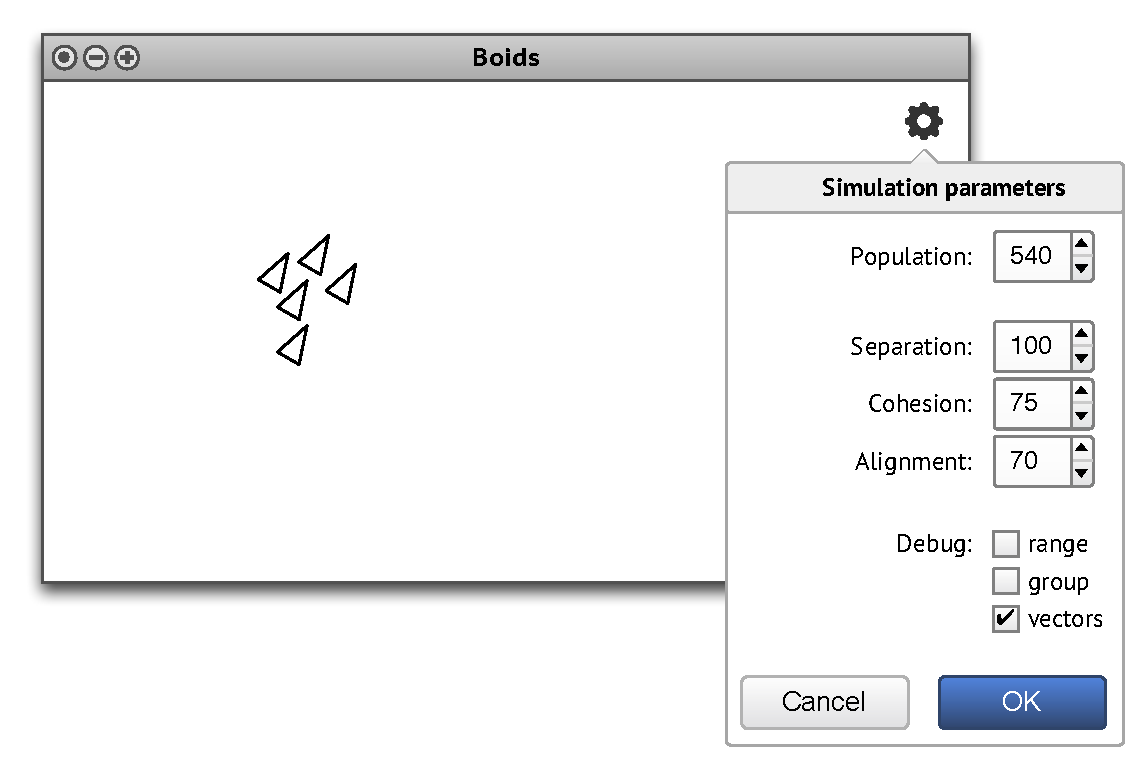
\includegraphics[scale=0.8]{./figury/wireframe}
    \caption{Szkic okna programu z widocznym menu parametrów symulacji.}
    \label{fig:wireframe}
\end{figure}

\subsection{Dynamiczna zmiana parametrów symulacji}
Program będzie umożliwiał zmianę zachowania symulowanej chmary. Podczas
modyfikacji parametrów symulacja będzie wstrzymywana.

Zmiana zachowania chmary polega na dostosowaniu wag każdej z trzech sił
działających na osobniki chmary. Siły te są wyszczególnione w \cite{reynolds}.
Możliwa też będzie zmiana liczby osobników w chmarze. Nowe osobniki pojawiać się
będą z losowym położeniem i zwrotem. Osobniki usuwane będą w kolejności
dodania do chmary.

\subsection{Rysowanie elementów debugujących}
Możliwe będzie wyświetlenie informacji sterujących osobnikami chmary w
symulacji. Wyświetlanie informacji jest aktywowane poprzez kliknięcie na
osobnika. Wyświetlane będą
\begin{enumerate}[nosep]
    \item zasięg wzroku osobnika,
    \item połączenia pomiędzy osobnikami, które uważają się za sąsiadów,
    \item wektory sił oddziałujących na osobnika i wektor wypadkowy.
\end{enumerate}
Chwilowo zakładamy, że wyświetlanie informacji będzie kosztowne wydajnościowo.
